\chapter{Metodologia}
\label{metodologia}

A elaboração dessa pesquisa utiliza como metodologias:

\begin{enumerate}
    \item[a)] Revisão bibliográfica - sobre o levantamento do estado da arte de conceitos relacionados a modelagem de \gls{DSL}s;
    
    \item[b)] Pesquisa documental - no que concerne à análise do histórico do controle de versão do \gls{IFSC} relacionando as alterações realizadas em função de documentos de lei ou em função de demandas dos envolvidos no processo de classificação de candidatos.
    
\end{enumerate}

Por fim, para avaliação desse estudo será realizado um experimento com os principais \textit{stakeholders} do IFSC envolvidos na definição de requisitos da lei. Essa avaliação visa identificar a usabilidade da \gls{DSL} proposta.

 \section{Classificação e etapas da pesquisa}
\label{natureza}

A elaboração do presente estudo caracterizou-se como uma pesquisa aplicada quanto à sua natureza. Segundo \citeonline{silva2005pesquisa}, a pesquisa aplicada visa gerar conhecimentos para aplicação prática e voltados à solução de problemas específicos e interesses locais.

Do ponto de vista da abordagem do problema a pesquisa classifica-se como qualitativa. Para \citeonline{silva2005pesquisa}, a pesquisa qualitativa preocupa-se com o processo de investigação, sendo que há uma relação dinâmica entre o objeto a ser estudado e o sujeito, estabelecendo-se um vínculo indispensável entre o mundo objetivo e a subjetividade do sujeito. Somada a essa questão, destaca-se que a interpretação dos fenômenos e a atribuição de significados pelo pesquisador é o instrumento-chave da pesquisa qualitativa.

Em relação aos objetivos, a pesquisa é exploratória, pois buscou:

\begin{citacao}
proporcionar maior familiaridade com o problema, com vistas a torná-lo mais explícito ou a constituir hipóteses[...] seu planejamento é, portanto, bastante flexível, de modo que possibilite a consideração dos mais variados aspectos relativos ao fato estudado \cite[p. 41]{gil2002elaborar}.
\end{citacao}

No que concerne aos procedimentos técnicos utilizou-se para o presente estudo: a pesquisa bibliográfica, a documental e o estudo de caso \cite{gil2002elaborar}. Esses procedimentos técnicos referem-se à:

\begin{enumerate}
    \item[a)] Pesquisa bibliográfica: realizada a partir de buscas aos documentos dos principais autores sobre \gls{DSL}: Fowler (2005, 2008) e Voelter (2011, 2013, 2014, 2018). A consulta aos referidos autores possibilitou a identificação de outros materiais sobre a temática, bem como outros pesquisadores utilizados no decorrer do texto. Ademais, utilizou-se a legislação sobre as leis de cotas no sistema de ensino público federal, que foram descritas no Capítulo \ref{chap:historicoversoes}. 

    
    \item[b)] Pesquisa documental: utilizada durante a análise do histórico do controle de versão do \gls{IFSC}, mediante à busca de \textit{commits} que contenham a palavra-chave "cotas" e a identificação dos arquivos envolvidos na classificação de candidatos. Nessa análise foram encontrados arquivos contendo as implementações das funcionalidades apresentadas no Capítulo \ref{chap:historicoversoes}, no qual foram detalhados as linhas de código e as funções envolvidas em 3 (três) versões do sistema de ingresso. 
    
    \item[c)] Estudo de caso: Para \citeonline{gil2002elaborar}, o estudo de caso tem o propósito de explorar situações da vida real no contexto do objeto estudado, buscando-se analisar e formular hipóteses sobre a sua aplicação. Por esses motivos foi utilizado nessa pesquisa articulando-se ao estudo de usabilidade da \gls{DSL}, baseado em \citeonline{nielsen2012many}. Para esse autor, quando o público alvo de usuários é variado, normalmente, os testes de usabilidade são realizados em grupos formados de 3 (três) a 4 (quatro) integrantes. Desse modo, considerando os objetivos da presente pesquisa, foram convidadas 20 pessoas com diferentes perfis de experiência, as quais responderam a um exercício proposto para desenvolvimento na \gls{DSL}, bem como a um questionário após a realização dos testes. 
    
\end{enumerate}

    O exercício na DSL (APÊNDICE X) e o questionário sobre a experiência de uso com os usuários (APÊNDICE Y), foram os instrumentos de coleta de dados utilizados na fase de validação de usabilidade. O perfil dos usuários, o detalhamento do exercício e o questionário serão retomados nas próximas Seções.
    
    Anteriormente à avaliação com os usuários foi realizado o desenvolvimento da DSL Cotas, assim como a sua validação por meio de seleção aleatória de 16 processos seletivos presentes na base do sistema de ingresso do \gls{IFSC}, conforme listados na Tabela \ref{processos_utilizados}. Esses processos possuem um total de 13494 candidatos classificados em primeira chamada no sistema de ingresso no período de 2013 até 2020, os quais foram utilizados para comparação de resultados de uma \gls{API} desenvolvida com base na DSL Cotas que foram descritas no Capítulo \ref{chap:dslcotas}.
    
    \begin{table}
\caption{Processos utilizados para avaliação da API}
\label{processos_utilizados}
\centering
\begin{tabular}{ |l| }
 \hline
2013/1 - Cursos Técnicos Integrados                                                        \\ \hline
2013/1 - Cursos Técnicos Concomitantes                                                     \\ \hline
2013/1 - Cursos Técnicos Subsequentes                                                      \\ \hline
2013/2 - Curso Técnico Subsequente - Palhoça - Edital 05/2013/2                            \\ \hline
2014/1 - Cursos Técnicos Integrados - Edital 01/DEING/2014/1                               \\ \hline
2014/1 - PROEJA/Técnico - Edital 06/DEING/2014/1                                           \\ \hline
2015/2 - Cursos de Graduação - Edital 04/DEING/2015-2                                      \\ \hline
2016/1 - Cursos Técnicos - Sorteio - Edital 05/DEING/2016/1                                \\ \hline
2016/1 - Cursos Técnicos Integrados - Exame de Classificação - Edital 01/DEING/2016/1      \\ \hline
2017/1 - Cursos Técnicos - Integrados e Concomitantes - Edital 01/DEING/2017/1             \\ \hline
2018/1 - Cursos Técnicos - Edital 07/DEING/2018/1 - Subsequentes e Concomitantes \\ \hline
2018/1 - Graduação - SiSU - Edital 13/DEING/2018/1                                         \\ \hline
2018/2 - Técnicos Itajaí - Sorteio - Edital 02/DEING/2018/2                                \\ \hline
2019/1 - Técnicos Integrados - Exame de Classificação - Edital 08/DEING/2019/1             \\ \hline
2019/1 - Cursos Técnicos - Sorteio - Edital 11/DEING/2019/1 - Integrados                   \\ \hline
2020/1 - Cursos Técnicos - Sorteio - Edital 15/DEING/2020/1 - Subsequentes                 \\ \hline
 \end{tabular} 
  \par\medskip\textbf{Fonte:} Base de dados do IFSC (2020). \par\medskip
\end{table}

    
    \newpage
    A fim de situar o leitor acerca das etapas desenvolvidas na pesquisa, apresenta-se a Figura \ref{fig:etapas}.
    
    
    \begin{figure}[ht!]
\centering

\caption{\textmd{Etapas da pesquisa}}
\label{fig:etapas}
\fcolorbox{gray}{white}{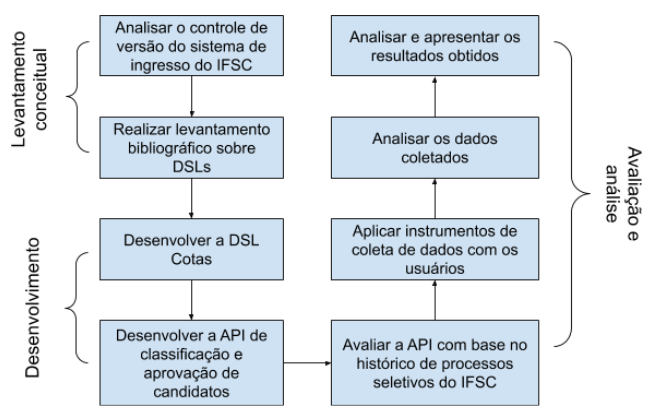
\includegraphics[width=0.76\textwidth]{chapters/metodologia/imagens/etapas.png}}

\par\medskip\textbf{Fonte:} Elaborada pelo autor (2020). \par\medskip

\end{figure}

    
    Com o intuito de apresentar os procedimentos metodológicos relativos ao ambiente da pesquisa, a Seção \ref{ambiente} descreve a metodologia de avaliação da DSL, abordando o perfil dos usuários, o detalhamento do exercício, o questionário aplicado e os critérios utilizados para avaliação da \gls{API}. 
    
    
    
  
 
 \section{Etapas de pesquisa}
\label{etapas}
 
 \section{Ambiente da pesquisa}
\label{ambiente}
 Este Capítulo apresenta o ambiente elaborado para verificar a validade da DSL de Cotas em relação aos objetivos da presente pesquisa. Desse modo, são descritos os critérios utilizados para definir os grupos de usuários convidados, os critérios de avaliação da \gls{API} implementada para classificar e aprovar os candidatos, e também apresentar o questionário aplicado com os participantes.
 
\subsection{Metodologia de avaliação da DSL}
\label{metododsl}

 Segundo \citeonline{kateMoran2018}, estudos qualitativos de usabilidade tentam compreender o pensamento e as dificuldades vivenciadas pelos indivíduos, geralmente este tipo de estudo apresenta aos usuários atividades abertas que têm o potencial de expor problemas na interface do sistema. 
 
 \citeonline{kateMoran2018} também cita alguns princípios básicos para elaboração de tarefas para qualquer tipo de teste com usuário, tais como:
 
 \begin{enumerate}
    \item[a)] Atente-se ao que seus usuários precisam fazer com o seu produto para inspirar suas tarefas;
    \item[b)] Evite fornecer dicas para a sua tarefa. Não descreva os passos exatos que o usuário precisa fazer, deixe que eles descubram por si só;
    \item[c)] Sempre faça um teste piloto para as tarefas, isso é essencial para evitar obter acidentalmente dados incorretos ou ruins.
    
\end{enumerate}
 
 Considerando essas orientações foi realizado um teste piloto da \gls{DSL} em Abril de 2020. Para tanto, foi instalado o software \textit{TeamViewer} para acesso remoto a uma máquina virtual \textit{Linux} contendo a ferramenta \gls{MPS}, no qual a DSL foi disponibilizada para teste. Todavia, observou-se que a ferramenta de acesso remoto dificultava o uso da linguagem, no sentido de apresentar lentidão durante a execução dos comandos. Outro problema percebido foi a falta de instruções sobre o uso da linguagem, bem como foram encontradas dificuldades de visualização de alguns elementos, tendo em vista que a fonte fornecida era pequena.
 
 A partir dessa avaliação foram feitas as correções necessárias, por meio da troca da ferramenta de acesso remoto para o software \textit{VNCViewer} e a elaboração de um documento para subsidiar os usuários. Desse modo, foi elaborado um manual de utilização da DSL (APÊNDICE X), no qual foram apresentados os objetivos e os elementos da linguagem, os principais comandos para edição das regras de negócio e o link para o vídeo explicativo também elaborado pelo autor, no qual se exibiu um exemplo de uso das principais funcionalidades. O ambiente para avaliação da DSL pode ser observado na Figura \ref{ambiente}.
 
 
  \begin{figure}[ht!]
\centering

\caption{\textmd{Ambiente de avaliação no \gls{MPS}}}
\label{fig:ambiente}
\fcolorbox{gray}{white}{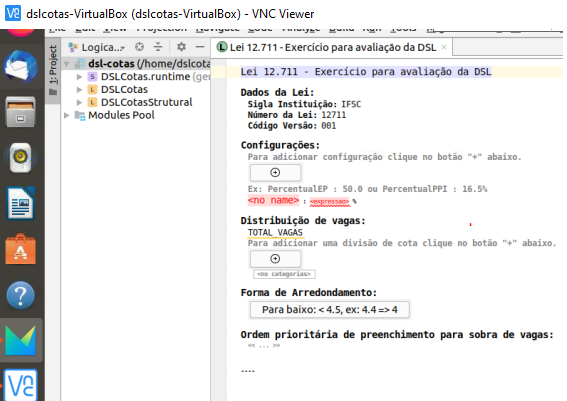
\includegraphics[width=0.76\textwidth]{chapters/metodologia/imagens/ambienteimg.png}}

\par\medskip\textbf{Fonte:} Elaboração do autor (2020) \par\medskip

\end{figure}


 
 No que concerne à seleção dos usuários para os testes, baseando-se em \citeonline{nielsen2012many}, entre os meses de Abril e Maio de 2020 buscou-se 20 pessoas com perfis diferentes que foram agrupadas de acordo com as seguintes categorias: 1) não desenvolvedores e especialistas na legislação de cotas; 2) desenvolvedores e não especialistas na legislação de cotas; 3) desenvolvedores e especialistas na legislação de cotas; 4) não desenvolvedores e não especialistas na legislação de cotas. Ao longo da análise dos dados estas foram identificadas no texto, respectivamente, como: NDEV-ESP; DEV-NESP; DEV-ESP; NDEV-NESP. 

 A coleta de dados iniciou-se por meio de envio de e-mail (APÊNDICE X) para cada participante, no qual constavam o manual de utilização da DSL, a instrução para acesso remoto, o link para o vídeo explicativo, e o exercício aberto para descrição da primeira versão de lei Nº 12.711 na DSL Cotas (Capítulo \ref{chap:historicoversoes}, Seção \ref{versao1}). Também foi sugerido para que os participantes contabilizassem o tempo utilizado para desenvolvimento do exercício. A instrução final do e-mail continha o link de acesso ao questionário de avaliação (Figura \ref{fig:questionario2}). O detalhamento completo do questionário, assim como as perguntas avaliadas estão presentes no Capítulo \ref{chap:analise} desse documento.

 \begin{figure}[ht!]
\centering

\caption{\textmd{Questionário aplicado}}
\label{fig:questionario2}
\fcolorbox{gray}{white}{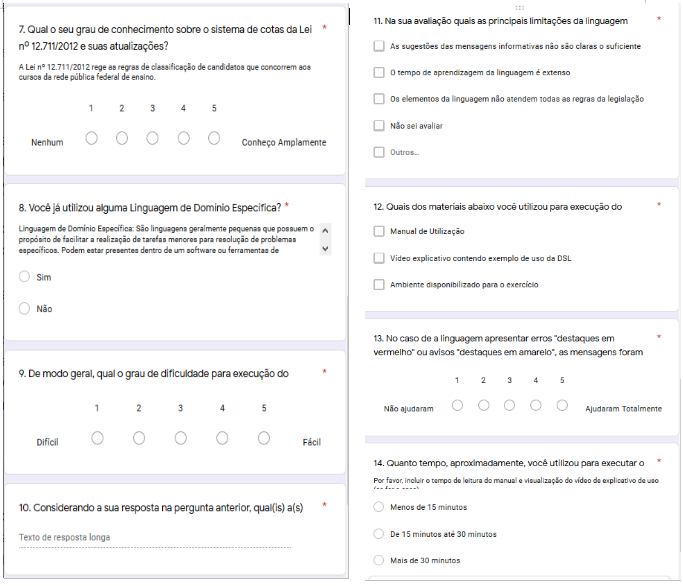
\includegraphics[width=1.00\textwidth]{chapters/metodologia/imagens/questionario2.png}}

\par\medskip\textbf{Fonte:} Elaborada pelo autor (2020). \par\medskip

\end{figure}

 
 \newpage
 Por fim, a Seção \ref{avaliacaoapi} descreve os procedimentos metodológicos criados de modo a possibilitar a avaliação da \gls{API}.
 

\subsection{Metodologia de avaliação da API}
\label{metodoapi}
Tendo como base a \gls{AST} da DSL elaborada, uma \gls{API} foi desenvolvida para disponibilizar \textit{endpoints} responsáveis pelos métodos de classificação e aprovação de candidatos. Para tanto, as regras definidas na linguagem foram exportadas em formato JSON o qual foi utilizado no framework \textit{SpringBoot} \footnote{Segundo \citeonline{springbootreference} o Spring Boot é um projeto da Spring que visa simplificar a criação de aplicativos Java com base no Spring \textit{Framework}, para que se tenha uma aplicação inicial sem a necessidade de muitas configurações.} para geração das operações \gls{API}. 

Desse modo, foi possível executar a classificação dos candidatos e fazer a comparação com os resultados de 13494 candidatos presentes na base de dados do sistema de ingresso em 16 processos seletivos selecionados aleatoriamente entre as diferentes versões de lei nas quais foram feitas classificações pelas regras de cotas. Para documentar as divergências entre os resultados da \gls{API} e o histórico presente no banco de dados do sistema, utilizou-se o recurso de \textit{issues} disponível no sistema de controle de versão \textit{github} (Figura \ref{fig:issues}). Para cada curso com diferenças nas situações de classificações, foi descrita a versão de lei aplicada na classificação, a quantidade de vagas, o problema apresentado, o motivo encontrado e uma possível solução.

\begin{figure}[ht!]
\centering

\caption{\textmd{Issues da \gls{API} no GitHub}}
\label{fig:issues}
\fcolorbox{gray}{white}{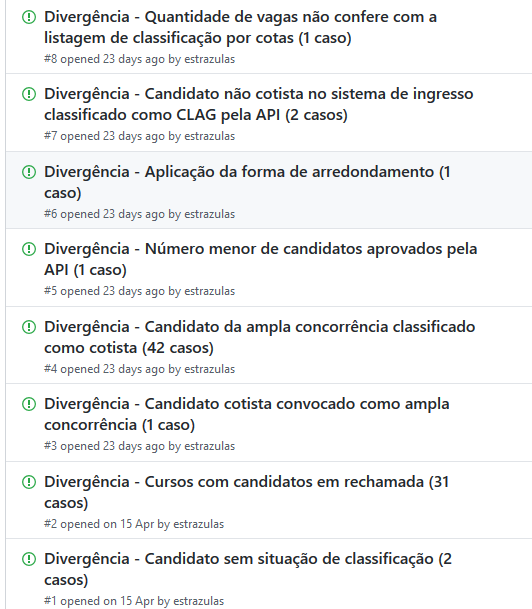
\includegraphics[width=0.70\textwidth]{chapters/metodologia/imagens/issues.png}}

\par\medskip\textbf{Fonte:} Elaborada pelo autor (2020). \par\medskip

\end{figure}



O detalhamento completo de implementação da \gls{API} é descrito no Capítulo \ref{chap:dslcotas} e a análise das divergências encontradas está presente no Capítulo \ref{chap:analise}. Por fim, no próximo Capítulo estão presentes os principais conceitos encontrados na literatura que serviram como base para fundamentar o desenvolvimento dessa pesquisa.
 